%%%%%%%%%%%%%%%%%%%%%%%%%%%%%%%%%%%%%%%%%%%%%%%%%%%%%%%%%%%%%%%%%%%%%%%%%%%%%%%%%%
\begin{frame}[fragile]\frametitle{}
\begin{center}
{\Large Introduction to Patanjali Yog-Sutra}
\end{center}
\end{frame}

%%%%%%%%%%%%%%%%%%%%%%%%%%%%%%%%%%%%%%%%%%%%%%%%%%%%%%%%%%%
 \begin{frame}[fragile]\frametitle{Patanjali  पतञ्जलि }
 
    \begin{columns}
    \begin{column}[t]{0.4\linewidth}
	
\begin{center}
\includegraphics[width=0.5\linewidth,keepaspectratio]{images/yog15}
\end{center}

\begin{sanskrit}
योगेन चित्तस्य पदेन वाचां |
मलं शरीरस्य च वैद्यकेन |
योऽपाकरोक्तं प्रवरं मुनीनां |
पतञ्जलिं प्राञ्जलिरनतोस्मि ||
- राजा भर्तुहरि
\end{sanskrit}

    \end{column}
    \begin{column}[t]{0.6\linewidth}
		\begin{itemize}
	\item Patajali has been mentioned to have 3 contributions (two of them are lost in time)
	\item Purification of mind (चित्तशुद्धि) using Yog $\rightarrow$ योगसूत्र 
	\item Purification of speech using Grammar  $\rightarrow$  महाभाष्य 
	\item Purification of body using medicine (Ayurveda)  $\rightarrow$  चरकसंहिता (?)
	\item Better amongst sages, we salute Rishi Patanjali
	\end{itemize}

    \end{column}
  \end{columns}
\end{frame}

%%%%%%%%%%%%%%%%%%%%%%%%%%%%%%%%%%%%%%%%%%%%%%%%%%%%%%%%%%%
\begin{frame}[fragile]\frametitle{Maharshi Patanjali महर्षि पतञ्जलि}

	\begin{itemize}
	\item Considered as `the father of Yoga'.
\item Many believe he’s thought to have lived between 200 and 500 B.C. 
\item At the time when the Ayurveda was the greatest wisdom, people had to cure their illness.	
\item Since, being sick it is not just sickness in the body, but also the sickness in the mind and emotions. 
\item The Yoga Sutras of Patanjali projects the knowledge that doesn’t just cure the body but also purify the mind, emotions and the complete existence itself, all through Yoga.
	\end{itemize}

\tiny{(Ref: Basic Introduction of Patanjali Yoga Sutras – The Best Knowledge for Yogis - Yoga Moha)}

\end{frame}

%%%%%%%%%%%%%%%%%%%%%%%%%%%%%%%%%%%%%%%%%%%%%%%%%%%%%%%%%%%
\begin{frame}[fragile]\frametitle{Panini and Patanjali}

	\begin{itemize}
	\item Panini's rules of Sanskrit grammar (`Ashtadhyayi') are the first known work on linguistics
	\item Yoga was there for ages, but Patanjali saw that it had become too complex and diversified for anyone to grasp in a meaningful way. So, he codified all aspects of yoga into a certain format known as the Yoga Sutras. 
	\item Patanjali also did Ayurveda (`Patanjalatantra') and Sanskrit grammar (`Mahabhasya').
	\end{itemize}

\begin{center}
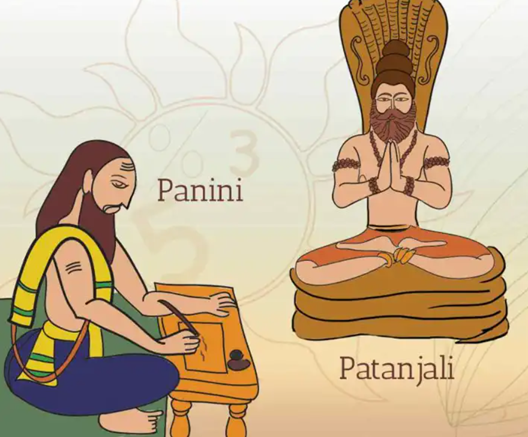
\includegraphics[width=0.3\linewidth,keepaspectratio]{images/patanjalipanini}
\end{center}


\tiny{(Ref: Sadhguru on Patanjali, Sushruta and Panini)}

\end{frame}



%%%%%%%%%%%%%%%%%%%%%%%%%%%%%%%%%%%%%%%%%%%%%%%%%%%%%%%%%%%
\begin{frame}[fragile]\frametitle{ योग सूत्र Yog Sutra}

	\begin{itemize}\item ``Yoga Sutra'': widely regarded as the authoritative text on `yoga'
	\item Collection Aphorisms, outlining the eight limbs of yoga.
	\item Sutras सूत्र (in Sanskrit) literally means a thread or string धागा that holds things together and more metaphorically refers to an aphorism	
	\item Guided by a single thread, a kite can glide and soar to amazing heights. 
	\item 	The Yoga Sutras of Patanjali are life’s threads, each one rich with knowledge, tools, and techniques. These sutras guide not only the mind but also one’s very being to its full potential. 
	\item 	Basically, Patanjali’s Yoga Sutras offer a systematic form of wisdom for attaining self-realization/enlightenment.
	\end{itemize}

\tiny{(Ref: Patanjali Yoga Sutra Dr Mrudula Chaudhari)}

\end{frame}


%%%%%%%%%%%%%%%%%%%%%%%%%%%%%%%%%%%%%%%%%%%%%%%%%%%%%%%%%%%
\begin{frame}[fragile]\frametitle{ योग सूत्र Yog Sutra}

	\begin{itemize}
	\item Minimum words, Unquestioned, Precise, essence, coherent eg. SthirSukhamAsan ( स्थिरसुखमासनम्| )
	\item Hard to understand by themselves so commentaries are needed.
	\item भाष्य commentaries starting with Vyas, are still going on (a living tradition)
	\item Vyasa's commentaries are highly regarded and have to be read along with Sutras.
	\end{itemize}

\tiny{(Ref: Patanjali Yoga Sutra Dr Mrudula Chaudhari)}

\end{frame}



%%%%%%%%%%%%%%%%%%%%%%%%%%%%%%%%%%%%%%%%%%%%%%%%%%%%%%%%%%%
\begin{frame}[fragile]\frametitle{Background}

	\begin{itemize}
	\item Patanjali Yog sutra emerged in the late Upanishad (उपनिषद) period
	\item Upanishads are earlier spiritual texts, but they are not systematic. They are mainly poetic expressions, metaphors some times confusing
	\item Examples: sometimes ब्रह्म साकार, sometimes ब्रह्म निराकार; जगन मिथ्या, जगन माया, जगन सत्य; आत्मन merges into ब्रह्मन्, etc). 
	\item Need to systematize.
	\end{itemize}

\tiny{(Ref: The Yoga Sutras of Patanjali | Prof. Edwin Bryant)}

\end{frame}

%%%%%%%%%%%%%%%%%%%%%%%%%%%%%%%%%%%%%%%%%%%%%%%%%%%%%%%%%%%
\begin{frame}[fragile]\frametitle{Systematization}

	\begin{itemize}
	\item Badarayana बादरायण codified unstructured Upanishad  उपनिषद texts.
	\item You get a few references to Yog in the Upanishads.
	\item Mentioned as techniques to attain ataman/brahman (आत्मन/ब्रह्मन्)
	\item Patanjali comes, systematizes and writes Yog Sutra (अथ अनुशाशन, continuing teachings of yog)
	\end{itemize}

\tiny{(Ref: The Yoga Sutras of Patanjali | Prof. Edwin Bryant)}

\end{frame}

%%%%%%%%%%%%%%%%%%%%%%%%%%%%%%%%%%%%%%%%%%%%%%%%%%%%%%%%%%%
\begin{frame}[fragile]\frametitle{Structure}

	\begin{itemize}
	\item Yogsutra has been divided into 4 chapters. `paad` (पाद) means foot, or quarter, as used while saying watch-timings (स+पाद, plus quarter). As there are 4 parts, each is called as a quarter.
	\item Total 195 verses/aphorisms
	\item Division:
		\begin{itemize}
		\item Samadhipad समाधिपाद 51
		\item Sadhanpad साधनपाद 55
		\item Vibhutipad विभूतिपाद 55
		\item Kaivalyapad कैवल्यपाद 34
		\end{itemize}	
	\end{itemize}

\tiny{(Ref: पातंजल योग सूत्र | Yog Darshan - Yoga And Ayurveda Science Youtube channel)}

\end{frame}

%%%%%%%%%%%%%%%%%%%%%%%%%%%%%%%%%%%%%%%%%%%%%%%%%%%%%%%%%%%
\begin{frame}[fragile]\frametitle{Contents}

Different Yogic methods for different types of people.

Types of people (prakruti प्रकृति ) in the world:

	\begin{itemize}
	\item High (uttam उत्तम ) : Already in almost pure mental state. Get success with very less efforts (sadhana !!!) 
	\item Medium (madhyam मध्यम )
	\item Low (adham अधम): Least pure mental state. Need vigorous discipline
	\end{itemize}
	
\tiny{(Ref: पातंजल योग सूत्र | Yog Darshan - Yoga And Ayurveda Science Youtube channel)}

\end{frame}

%%%%%%%%%%%%%%%%%%%%%%%%%%%%%%%%%%%%%%%%%%%%%%%%%%%%%%%%%%%
\begin{frame}[fragile]\frametitle{Contents}

Methods to attain yogic state based on type:


	\begin{itemize}
	\item Samadhipad समाधिपाद : , for uttam prakrti people, along with study (abhyas अभ्यास) and renunciation (vairagya वैराग्य)
	\item Sadhanpad साधनपाद : for adham prakriti people. Ashtang yog to get rid off miseries in life.
	\item Vibhutipad विभूतिपाद : After doing sadhana (dharana धारणा, dhyaan ध्यान, samadhi समाधि), one can get certain powers (siddhi सिद्धि, vibhuti विभूति). Recommends not get enamored by these powers.
	\item Kaivalyapad कैवल्यपाद : State of self detachment (moksh मोक्ष, mukti मुक्ति)
	\end{itemize}	

\tiny{(Ref: पातंजल योग सूत्र | Yog Darshan - Yoga And Ayurveda Science Youtube channel)}

\end{frame}


%%%%%%%%%%%%%%%%%%%%%%%%%%%%%%%%%%%%%%%%%%%%%%%%%%%%%%%%%%%
\begin{frame}[fragile]\frametitle{Contents}
	\begin{itemize}
	\item Yog Sutra is a practice text, and not a knowledge text.
	\item The Knowledge part is covered in Sankhya darshan (साङ्ख्य दर्शन)
	\item It is assumed that you have gone through the knowledge texts before.
	\item Gita's yoga definition is ACTION oriented, whereas Patanjali definition is IN-ACTION oriented.
	\end{itemize}

\tiny{(Ref: The Yoga Sutras of Patanjali | Prof. Edwin Bryant)}

\end{frame}

%%%%%%%%%%%%%%%%%%%%%%%%%%%%%%%%%%%%%%%%%%%%%%%%%%%%%%%%%%%
\begin{frame}[fragile]\frametitle{Primary References}
	\begin{itemize}
	\item On many slides you will find info with interpretations from different folks. They are from  site Yoga Sutra Study https://yogasutrastudy.info/
		\begin{itemize}
		\item [HA]: Hariharananda Aranya
		\item [IT]: I. K. Taimni
		\item [VH]: Vyasa Houston
		\item [BM]: Barbara Miller
		\item [SS]: Swami Satchidananda
		\item [SP]: Swami Prabhavananda
		\item [SV]: Swami Vivekananda
		\end{itemize}	
	\item Also, many slides will have Samskrit vigraha and [untagged] meaning, that's mainly from https://patanjaliyogasutra.in/
	\end{itemize}

Highly indebted for making such valuable information open.

\end{frame}

%%%%%%%%%%%%%%%%%%%%%%%%%%%%%%%%%%%%%%%%%%%%%%%%%%%%%%%%%%%
\begin{frame}[fragile]\frametitle{Commentaries}
    
    \begin{itemize}
        \item \textbf{Ved Vyasa}
        \begin{itemize}
            \item Authored the first and most authoritative commentary, known as the Vyasa Bhashya.
            \item Provides extensive explanations of the sutras, laying the foundation for subsequent interpretations.
            \item Emphasizes the philosophical underpinnings and the practical aspects of Yoga.
			\item Vachaspati Mishra (9th CE) wrote commentary on Vsyasa-bhashya called tatv-vaisharadi
        \end{itemize}
        
        \item \textbf{Raja Bhoja}
        \begin{itemize}
            \item Composed the Bhoja Vritti, a detailed and insightful commentary.
            \item Focuses on the integration of Yoga with other philosophical systems.
            \item Highlights the historical and cultural context of the sutras.
        \end{itemize}
        
        \item \textbf{Adi Shankara}
        \begin{itemize}
            \item Though primarily known for Advaita Vedanta, he also provided commentary on Yogasutra.
            \item Aligns the principles of Yoga with the non-dualistic approach of Advaita Vedanta.
            \item Emphasizes the unity of Atman and Brahman in the practice of Yoga.
        \end{itemize}
        
        \item \textbf{Swami Vivekananda}
        \begin{itemize}
            \item Modern interpreter who made the Yogasutra accessible to a global audience.
            \item His commentary in "Raja Yoga" simplifies complex concepts for contemporary readers.
            \item Emphasizes practical application and the psychological aspects of Yoga.
        \end{itemize}
    \end{itemize}
    
\end{frame}


%%%%%%%%%%%%%%%%%%%%%%%%%%%%%%%%%%%%%%%%%%%%%%%%%%%%%%%%%%%
\begin{frame}[fragile]\frametitle{Ref Card}

\begin{center}
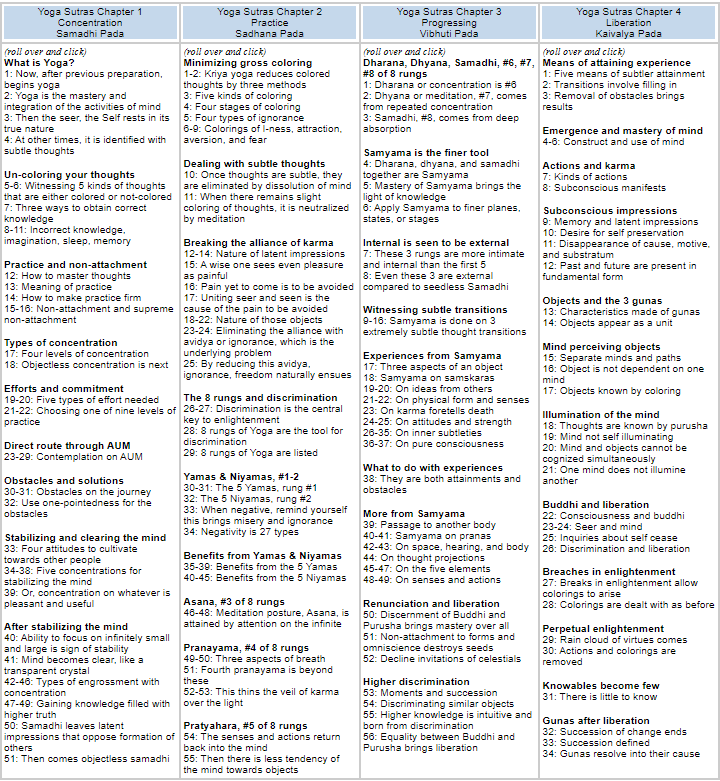
\includegraphics[width=0.6\linewidth,keepaspectratio]{SwamiJ_YogasutraCard}

\end{center}

  
  \tiny{(Ref: Yoga Sutras of Patanjali - Raja Yoga - Ashtanga Yoga - Swami J/Rama)}

\end{frame}


%%%%%%%%%%%%%%%%%%%%%%%%%%%%%%%%%%%%%%%%%%%%%%%%%%%%%%%%%%%
\begin{frame}[fragile]\frametitle{What are the Yoga Sutras?}

\begin{itemize}
\item Succinctly outlines art and science of Yoga meditation for Self-Realization
\item Systematically encountering and transcending levels of false identity in mind
\item Patanjali codified and compiled ancient practices in organized, terse way
\item Not a new system, but summarization of ancient practices
\item Thought to be as old as 400 BCE
\item Archaeological evidence suggests methods described were practiced as early as 3000 BCE
\item Oral tradition suggests even longer period
\item Process of examining and transcending gross and subtle levels of false identity
\item Until jewel of true Self shines through
\item Extremely organized and terse summarization of ancient practices
\end{itemize}

\begin{center}
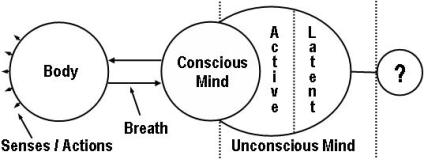
\includegraphics[width=0.4\linewidth,keepaspectratio]{yogaswamij1}

\end{center}

  
  \tiny{(Ref: Yoga Sutras of Patanjali - Raja Yoga - Ashtanga Yoga - Swami J/Rama)}

\end{frame}

%%%%%%%%%%%%%%%%%%%%%%%%%%%%%%%%%%%%%%%%%%%%%%%%%%%%%%%%%%%
\begin{frame}[fragile]\frametitle{Yoga means union \& sutra means thread}

\begin{itemize}
\item Yoga means union of parts of ourselves, never divided
\item Literally means to yoke, join, from the root "yuj"
\item Absorption in state of samadhi (union, enlightenment)
\item Sutra means thread, threads weave tapestry of insight and experience
\item Some say Sutras (plural) - each thread forms complete tapestry
\item Others say Sutra (singular) - one consistent thread through text
\item Both views provide useful perspective on process described
\item Union of parts refers to uniting different aspects of self
\item Never divided in first place, just perception of division
\item Direct experience and insight into true nature of reality
\end{itemize}

  
  \tiny{(Ref: Yoga Sutras of Patanjali - Raja Yoga - Ashtanga Yoga - Swami J/Rama)}

\end{frame}

%%%%%%%%%%%%%%%%%%%%%%%%%%%%%%%%%%%%%%%%%%%%%%%%%%%%%%%%%%%
\begin{frame}[fragile]\frametitle{Why Read the Yoga Sutras?}


\begin{center}
{\Large ``If you are on any path where you want to be happy, to be free of suffering, and understand the mind and consciousness, the Sutras are a must-read.''} – Edwin Bryant, Professor at Rutgers, PhD from Columbia
\end{center}

  

\end{frame}

%%%%%%%%%%%%%%%%%%%%%%%%%%%%%%%%%%%%%%%%%%%%%%%%%%%%%%%%%%%
\begin{frame}[fragile]\frametitle{Learning Path}

\begin{center}
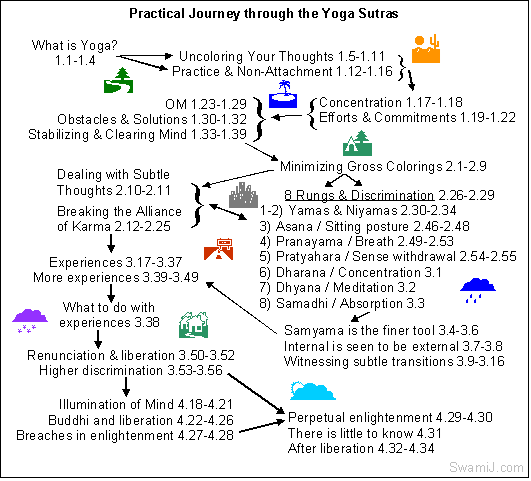
\includegraphics[width=0.6\linewidth,keepaspectratio]{SwamiJ_LearningPath}

\end{center}

  
  \tiny{(Ref: Yoga Sutras of Patanjali - Raja Yoga - Ashtanga Yoga - Swami J/Rama)}

\end{frame}

%%%%%%%%%%%%%%%%%%%%%%%%%%%%%%%%%%%%%%%%%%%%%%%%%%%%%%%%%%%
\begin{frame}[fragile]\frametitle{Yoga Achievement Paths}

\begin{itemize}
\item Original (ऋग्वेद ) meaning of 'Yoga' was connection, joining and also to 'control of horses', later it became 'control of senses'
\item Ancient India had many physical and mental practices in use. Patanjali may have systematized them and gave a philosophical form using सांख्य  basis. Thus it became part of 6 दर्शन .
\item Yoga is actually Indian Psychology, traces man's journey to a state which is free from afflictions (क्लेश ) and effects of कर्म  thus unfolding infinite knowledge.
\item Definition of सूत्र (aphorisms, verses) : अल्पाक्षरं असंदिग्धं सारवत्‌ विश्वतोमुखम्‌। अस्तोभं अनवद्यं च सूत्रं सूत्र विदो विदुः॥
\item Vyasa defines yoga not as joining but as समाधि  (सं + आ  + धि ,  equal balance + all around +  चित्त ), just आ  + धि is scattered चित्त which is a mental disease, remember the opposite word व्याधि (वि + आ + धि ) scattered चित्त which is a physical disease
\end{itemize}
  
  \tiny{(Ref: An Introduction to Patanjali’s Yoga Darshana - Dr Veena Londhe (Chinmay Mission course))}

\end{frame}

%%%%%%%%%%%%%%%%%%%%%%%%%%%%%%%%%%%%%%%%%%%%%%%%%%%%%%%%%%%
\begin{frame}[fragile]\frametitle{Yoga Achievement Paths}

\begin{itemize}
\item As per Vyasa, चित्त is a product of प्रकृति  thus it is त्रिगुणात्मक (सत्व, रजस , तमस )
\item 5 states of चित्त (चित्तभूमी)
	\begin{itemize}
	\item क्षिप्त  - dominance of  रजस – Chaotic or most fickle state of mind
	\item मूढ  – dominance of  तमस - Dull or Lazy state of mind
	\item विक्षिप्त  – occasional रजस and some सत्व – Partially focused mind
	\item एकाग्र   – dominance of  सत्व – One-pointed mind
	\item निरुद्ध  – Restrained  चित्त – Fully absorbed mind
	\end{itemize}
\end{itemize}
  
  \tiny{(Ref: An Introduction to Patanjali’s Yoga Darshana - Dr Veena Londhe (Chinmay Mission course))}

\end{frame}

%%%%%%%%%%%%%%%%%%%%%%%%%%%%%%%%%%%%%%%%%%%%%%%%%%%%%%%%%%%
\begin{frame}[fragile]\frametitle{Yoga Achievement Paths}

\begin{itemize}
\item For superior type of practitioners : अभ्यास  वैराग्य (१.१२)
\item For middle type of practitioners : क्रियायोग (२.१)
\item For ordinary type of practitioners : अष्टांग योग (२.२८)
\item For emotional type of practitioners: ईश्वर प्रणिधान  (१.२३)
\end{itemize}
  
  \tiny{(Ref: An Introduction to Patanjali’s Yoga Darshana - Dr Veena Londhe (Chinmay Mission course))}

\end{frame}


%%%%%%%%%%%%%%%%%%%%%%%%%%%%%%%%%%%%%%%%%%%%%%%%%%%%%%%%%%%
\begin{frame}[fragile]\frametitle{Other Names for Yoga}
\begin{itemize}
\item Raja Yoga (Royal Yoga)
\item Kriya Yoga (drawing on use of word 'Kriya' from Chapter 2)
\item Ashtanga Yoga (Eight-fold path of Yoga)
\item Includes yamas, niyamas, asana, pranayama, pratyahara, dharana, dhyana, samadhi
\item Begins with Sutra 28 of Chapter 2 (2.28)
\item Not referring to popularized physical yoga using same name
\item Ashtanga Yoga (Ashta = eight; anga = rungs)
\item Yamas (restraints), Niyamas (observances)
\item Asana (postures), Pranayama (breath control)
\item Pratyahara (withdrawal of senses), Dharana (concentration)
\item Dhyana (meditation), Samadhi (absorption, enlightenment)
\end{itemize}
  
  \tiny{(Ref: Yoga Sutras of Patanjali - Raja Yoga - Ashtanga Yoga - Swami J/Rama)}

\end{frame}

%%%%%%%%%%%%%%%%%%%%%%%%%%%%%%%%%%%%%%%%%%%%%%%%%%%%%%%%%%%
\begin{frame}[fragile]\frametitle{Key Yogic Concepts}
      \begin{itemize}
        \item \textbf{पुरुष (Purusha)}: The pure consciousness, eternal and unchanging.
        \item \textbf{प्रकृति (Prakriti)}: The primal matter, source of all creation.
        \item \textbf{चित्त (Chitta)}: The mind-stuff, including thoughts, memories, and emotions.
        \item \textbf{मनस (Manas)}: The sensory mind that processes perceptions.
        \item \textbf{बुद्धि (Buddhi)}: The intellect or faculty of discrimination.
        \item \textbf{अहंकार (Ahamkara)}: The ego, identifying self as separate.
        \item \textbf{जीवात्मा (Jivatma)}: The individual soul bound by material existence.
        \item \textbf{परमात्मा (Paramatma)}: The supreme soul or universal consciousness.
        \item \textbf{त्रिगुण: सत्व रजस तमस (Triguna: Sattva, Rajas, Tamas)}: Three qualities governing nature—purity, activity, inertia.
        \item \textbf{पञ्च महाभूत: (Pancha Mahabhuta)}: The five great elements—earth, water, fire, air, space.
        \item \textbf{त्रि दोषः (Tri Dosha)}: Three bodily humors—Vata, Pitta, Kapha.
        \item \textbf{सप्त धातु (Sapta Dhatu)}: The seven bodily tissues—plasma, blood, muscle, fat, bone, marrow, reproductive essence.
      \end{itemize}
\end{frame}

%%%%%%%%%%%%%%%%%%%%%%%%%%%%%%%%%%%%%%%%%%%%%%%%%%%%%%%%%%%
\begin{frame}[fragile]\frametitle{Key Yogic Concepts}
      \begin{itemize}
		\item \textbf{धि} is mind, \textbf{आधि} is anxious mind \textbf{व्याधी } is disturbed mind ie disease, can be due to:
		\begin{itemize}
			\item \textbf{आधिभौतिक (Adhibhautika)}: Suffering caused by external factors.
			\item \textbf{आधिदैविक (Adhidaivika)}: Suffering due to natural or divine forces.
			\item \textbf{अध्यात्मिक (Adhyatmika)}: Suffering originating within oneself.
		\end{itemize}

      \end{itemize}
\end{frame}
